% !TEX TS-program = xelatex
% !TEX encoding = UTF-8 Unicode
% !Mode:: "TeX:UTF-8"

\documentclass{resume}
\usepackage{zh_CN-Adobefonts_external} % Simplified Chinese Support using external fonts (./fonts/zh_CN-Adobe/)
%\usepackage{zh_CN-Adobefonts_internal} % Simplified Chinese Support using system fonts
\usepackage{linespacing_fix} % disable extra space before next section
\usepackage{cite}
\usepackage{graphicx}
\usepackage{tabularray}

\begin{document}
\pagenumbering{gobble} % suppress displaying page number

\name{江锋}

\begin{tblr}
  { 
      width             = \textwidth, 
      colspec           = {X[1,l]X[3,l]X[1,l]},
      cell{1}{3}        = {r=4,c=1}{c,m},
  }
  \textbf{学{\quad}{\quad}历} & 浙江大学 (博士,C9) + 大连理工大学 (本科,985) & 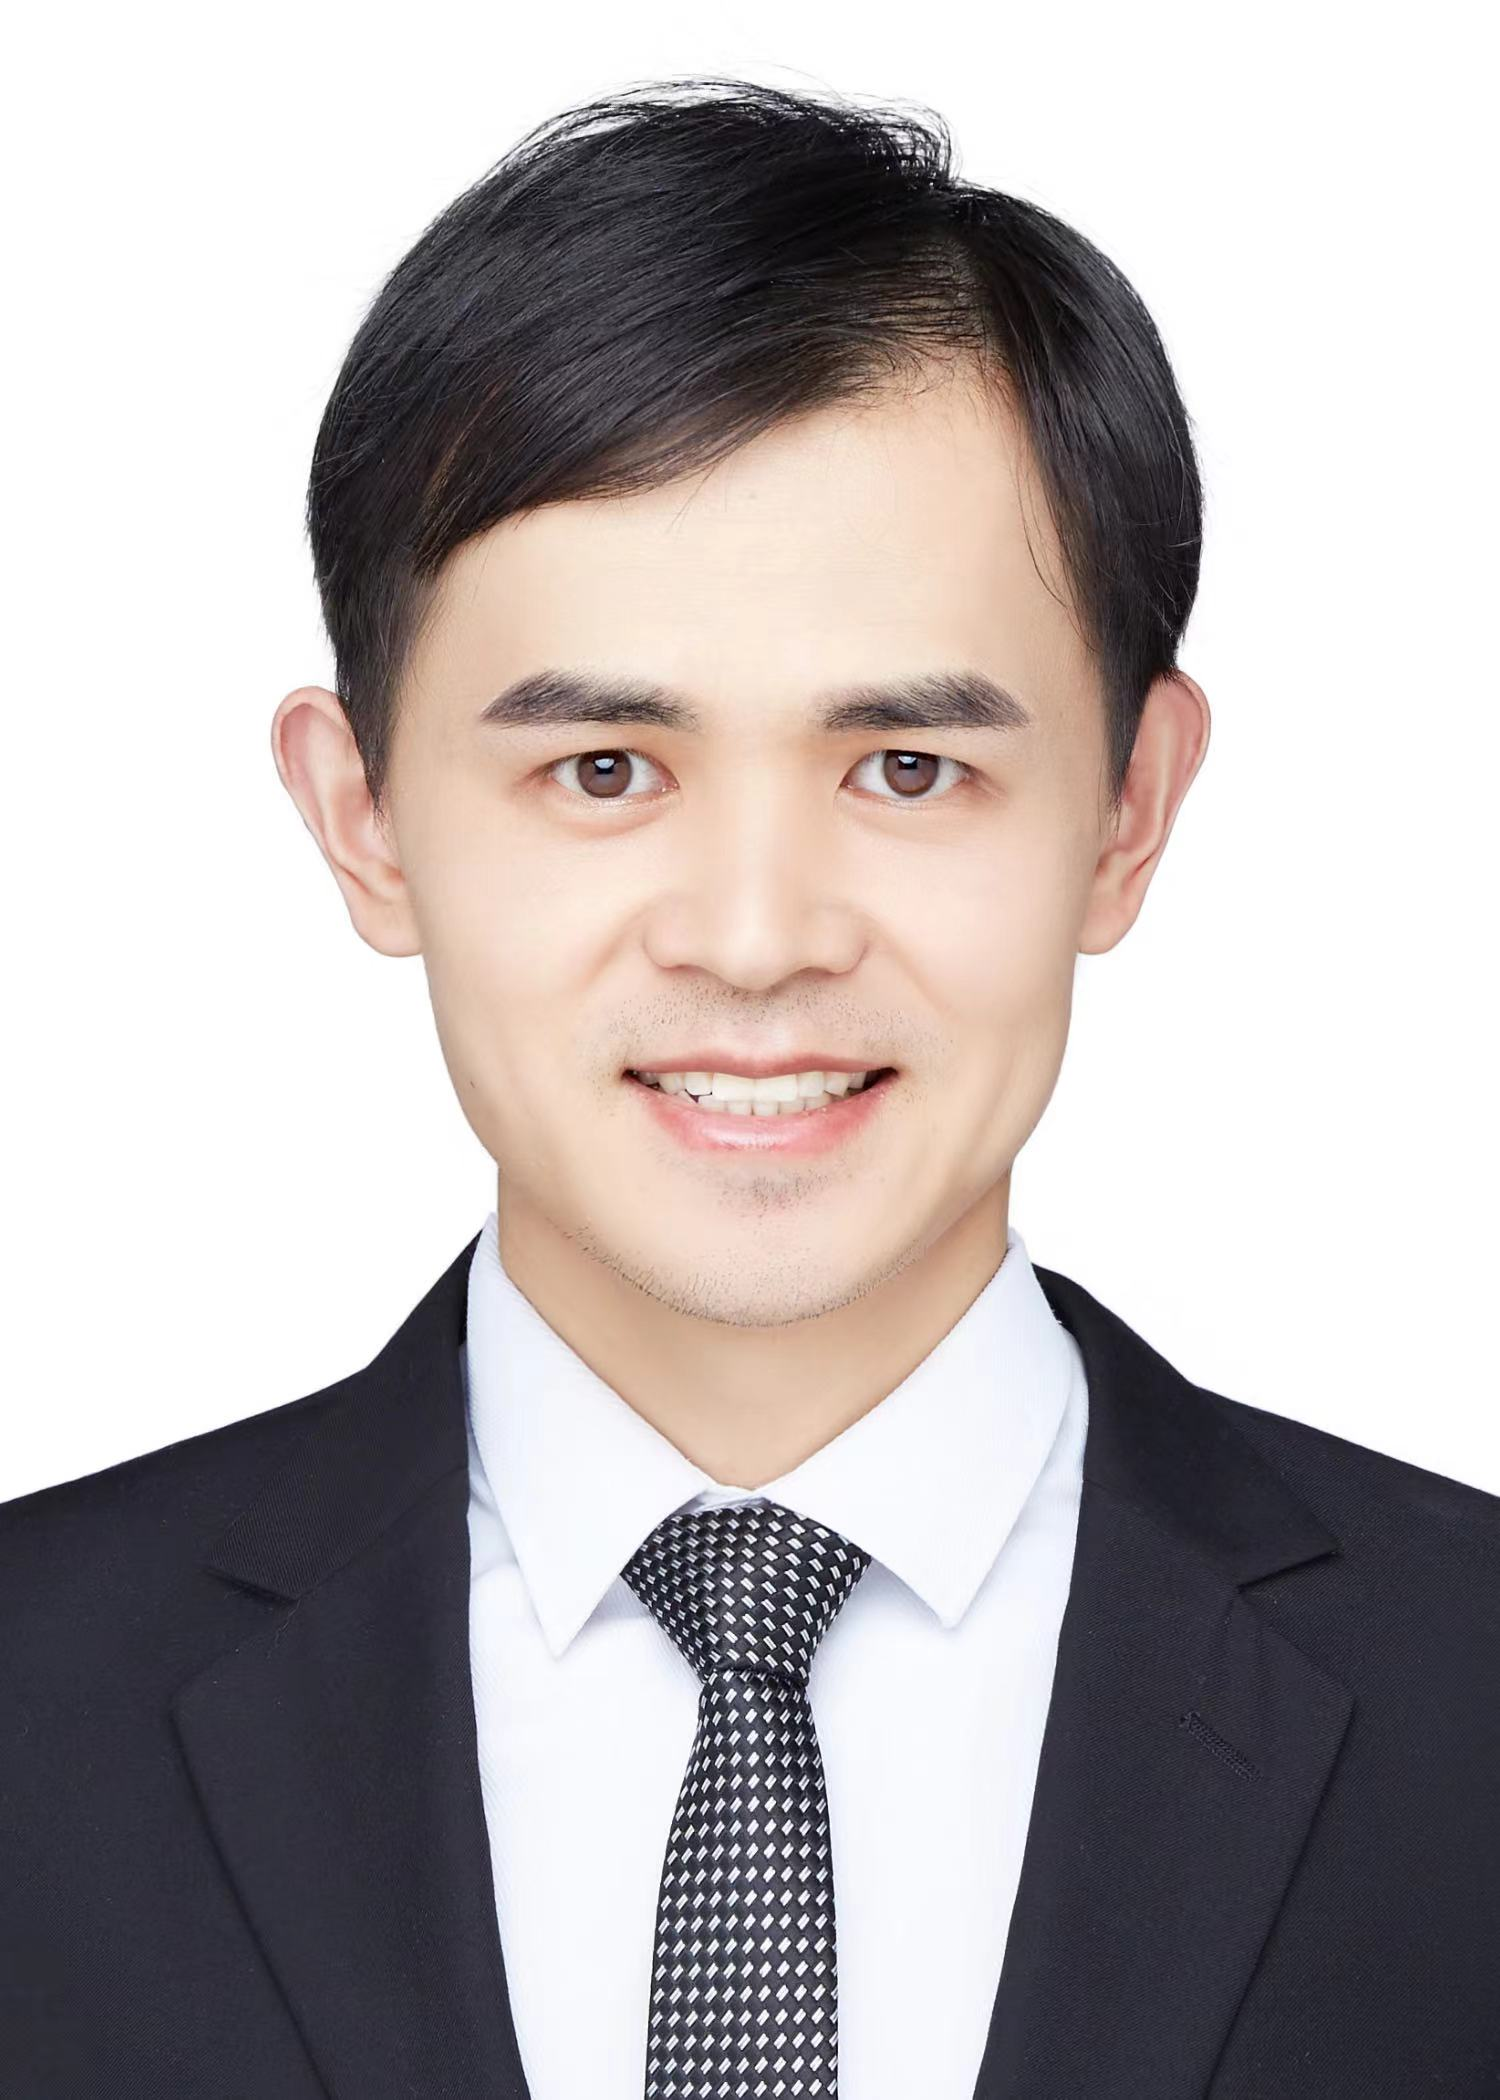
\includegraphics[width=1.6cm]{figures/2020}\\
  \textbf{研究方向} & 医学信号分析处理、嵌入式研发  & \\
  \textbf{手机/微信} & 159 6715 7216   &   \\
  \textbf{邮{\quad}{\quad}箱}& silencejiang@zju.edu.cn &  \\
  \textbf{GitHub} & @xfz329 \\
\end{tblr}

% {E-mail}{mobilephone}{homepage}
% be careful of _ in emaill address
% \contactInfo{医学信号分析处理}{159-6715-7216}{silencejiang@zju.edu.cn}{GitHub @xfz329}
% {E-mail}{mobilephone}
% keep the last empty braces!
%\contactInfo{xxx@yuanbin.me}{(+86) 131-221-87xxx}{}

% \section{}
% \datedsubsection{\textbf{}, }{2018.11-2019.1}
% \begin{itemize}
%     \item 
%     \item 
% \end{itemize}

% \section{\faGraduationCap\ 教育背景}
\section{教育背景}
\datedsubsection{\textbf{浙江大学},生物医学工程专业,嵌入式及人体电生理信号处理方向,\textit{硕博连读}}{2015.09-2024.03}
\begin{itemize}
    \item \textbf{主修课程:}生物医学工程方法学、数字图像处理、生物医学信号处理、微机系统设计与开发、现代医学仪器、
    生物医学仪器的嵌入式软件等
    \item \textbf{获得荣誉:}优秀博士岗位助学金,优秀研究生,三好研究生;生仪学院优秀学生党支部书记,优秀研究生干部
\end{itemize}
\datedsubsection{\textbf{大连理工大学},生物医学工程专业,\textit{本科}}{2010.09-2014.06}
\begin{itemize}
    \item \textbf{主修课程:}模拟电路基础、数字电路基础、C语言、数据结构、通信原理、数字信号处理、微机原理、医学成
    像技术与图像处理、医学信号分析与处理等
    \item \textbf{获得荣誉:}全国首届生物医学电子创新设计大赛自选项目组二等奖,2014年8月
\end{itemize}

\section{项目经历}
\datedsubsection{\textbf{临床麻醉深度评估指标PK值的研究}}{2023.01-2023.09}
\textbf{项目介绍:}改进了广泛使用的临床麻醉指标值PK值(\textit{Measuring the Performance of Anesthetic Depth Indicators},W D.Smith,Anesthesiology,IF=8.8,Cites=582)的计算方式,
分别开发了R语言与Python的软件包,得到了原作者的授权与肯定
\begin{itemize}
    \item 基于R语言,完成了PK计算软件包pk4adi的开发,2023年7月已被R语言官方仓库CRAN收录
    \item 基于Python,分别完成了PK计算软件的CLI版本(pk4adi)与GUI版本(pk4adi\_calculator)的开发,GUI版本支持选择文件一次性评估比较多个参数,两者均已在Github上开源
    \item 工作内容与成果得到原作者的授权与高度肯定,相关成果整理投稿中
\end{itemize}
\datedsubsection{\textbf{基于光电容积脉搏波PPG的子痫前期PE识别模型的研究},博士毕业论文课题}{2017.09-2022.12}
\textbf{项目介绍:}在临床PE患者与正常孕妇人群PPG数据的基础上,探索分析PE对PPG波形的影响与借助PPG波形识别PE的可能性;
设计了多种PPG时域形态学特征参数;通过机器学习的方法,建立了具有一定识别效果的PE识别模型;设计并实现了模块化的PE识别分析的综合软件系统
\begin{itemize}
  \item 与临床医生合作,完成基本数据的采集工作
  \item 基于Qt,完成了实验室自研多生路生理信号采集设备的上位机软件研发,具有USB数据通讯、数据保存、实时绘图等功能
  \item 提出了一种新型PPG波形检测算法SCD,可依据信号质量进行定制,相较其他算法而言,对包含异常PPG波形的检测准确率具有性能优势
  \item 提出了多种PPG新型形态学时域特征,构建了PPG波形的描述特征参数集合
  \item 基于Sklearn,使用多种机器学习算法构建了PE识别模型,经测试,所得模型具有一定的PE识别能力
  \item 设计并实现了模块化的PE识别分析的综合软件系统,包括基于Java的数据与处理模块、基于Java的跨平台(PC与Android)客户端模块、基于Sklearn的PE识别模型训练模块与
  基于Django的云服务器等模块,经测试,可按预期正常运行,具有一定的应用前景
  \item 目前已完成\textbf{4}篇文章的发表,\textbf{1}篇SCI在投中,另有\textbf{1}篇文章整理撰写中,\textbf{1}项软件著作权申请中
\end{itemize}
\datedsubsection{\textbf{基于人体心冲击图BCG的智能睡眠床垫系统的研发}}{2016.01-2016.10}
\textbf{项目介绍:}设计集成于智能床垫的能够采集BCG的嵌入式微机采集系统,采集受试者的ECG与BCG睡眠数据,并以此分
析受试者的睡眠状况
\begin{itemize}
  \item 负责基于STM32F411芯片的ECG与BCG两路生理信号采集系统的嵌入式软件设计
  \item 负责系统串口通讯协议设计与现实,完成TF卡本地存储及串口发送等数据保存与通讯功能
  \item 负责两路电生理信号的预处理,对两路信号的一致性进行了验证
\end{itemize}

\section{实习经历}
\datedsubsection{\textbf{浙江省杭州市特种设备检测研究院},软件开发工程师}{2019.04-2019.06}
\begin{itemize}
    \item 基于百度的OCR云技术,完成了针对特种材料焊接工艺评定及焊接操作人员资质解读的Android软件开发
    \item 可选择相机或直接对本地图片中资质信息进行解读,提供资质代号信息的自然语言翻译,提供人工校正功能
    \item 以Android设备的网卡地址信息为基础,实现了软件使用权限的申请管理,保证了软件使用范围的可控性
\end{itemize}
\datedsubsection{\textbf{浙江雅锐斯智能科技有限公司},软件开发工程师}{2018.11-2019.01}
\begin{itemize}
    \item 使用Java/Servlet开发了收发HTTP访问请求并操作可编程逻辑控制器PLC的中间应用服务程序
    \item 软件接收请求命令,通过FINS协议访问操作PLC设备,转发PLC执行结果至HTTP请求端
    \item 已在公司全自动中药配方颗粒调剂系统、智能实时打印贴标机等产品上正式投入使用
\end{itemize}
\datedsubsection{\textbf{浙江千成电子科技有限公司},软件开发工程师}{2015.04-2015.09}
\begin{itemize}
    \item 负责公司单道动态心电记录仪的低功耗蓝牙BLE通讯模块的嵌入式软件设计
    \item 负责公司Android端APP的设计开发,实现了与单通道心电记录仪的BLE通讯,具有心电数据的实时显示、数
    据转存、基本心电事件检测分析等功能
\end{itemize}

\section{科研成果}
\textbf{SCI}
\begin{itemize}
  \item \textit{A novel parameter derived from photoplethysmographic pulse wave to distinguish preeclampsiafrom
  non-preeclampsia},Pregnancy Hypertension:An International Journal of Women's Cardiovascular Health,IF=2.49,2019 
  \item \textit{Distinguishing preeclampsia using the falling scaled slope(FSS), a novel photoplethysmographic morphological parameter},
  Hypertension in Pregnancy,IF=2.00,2023 
\end{itemize}
\textbf{EI}
\begin{itemize}
  \item \textit{The Research of Photoplethysmography Morphology: Distincting Preeclampsia with Hierarchical Area Ratio},
  2018 The 3rd International Conference on Information Communication and Signal Processing of IEEE,2018 
  \item \textit{一种基于新型检测算法的模块化的脉搏波预处理分析系统的设计与实现},《生物医学工程学杂志》,2023 
\end{itemize}

\section{技术能力}
% increase linespacing [parsep=0.5ex]
\begin{itemize}[parsep=0.2ex]
  \item \textbf{算法:} 熟悉树、图、栈等常见数据结构的基本算法,熟悉信号处理方向的常见算法,熟悉机器学习的常见算法,熟悉常见的机器学习的算法原理
  \item \textbf{编程语言:} 熟悉Matlab,Java/Android,C/C++,Shell/Makefile,Python,R等编程语言
  \item \textbf{嵌入式开发:} 具有 ARM LPC1700、STM32F 系列等芯片的开发经验,熟悉串口、蓝牙、USB等通讯软件的开发
流程, 有在此基础上自定义通讯协议的开发设计经验
  \item \textbf{操作系统:} 熟悉Linux,熟悉操作系统的相关概念,熟悉嵌入式实时系统μCOS
  \item \textbf{工程构建:} 熟悉Design Pattern相关原理,熟悉Git与Github
  \item \textbf{写作能力:} 扎实的中英文写作能力,良好的技术文档写作能力,良好的编码写作习惯
  \item \textbf{外语能力:} 熟练的英文文献与技术文档阅读能力,CET6
\end{itemize}

\section{个人总结}
本人在校期间成绩优秀,乐观向上,工作负责,自我驱动能力强,热爱尝试新事物,学习能力强。
勇于接受挑战,享受解决问题的过程与攻克之后的成就感
% 在校期间由于
% 科研需要与兴趣驱动,一直从事人体电生理信号的研究相关工作,熟悉相关信号的基本产生采集原理,熟悉嵌入
% 式软件的设计及上位机软件的基本开发流程,熟悉基本包括Uart、BT、BLE、USB等电子电路的相关通讯协议的
% 原理及基本通讯软件的研发,熟悉生物医学信号处理的基本流程。看好医疗健康领域的发展趋势并有志于投身医
% 疗健康仪器设备的开发设计的关系国计民生的事业中
%% Reference
%\newpage
%\bibliographystyle{IEEETran}
%\bibliography{mycite}
\end{document}
